%{{{ Formatierung

\documentclass[a4paper,10pt]{article}

\usepackage{physics_notetaking}

%%% dark red
%\definecolor{bg}{RGB}{60,47,47}
%\definecolor{fg}{RGB}{255,244,230}
%%% space grey
%\definecolor{bg}{RGB}{46,52,64}
%\definecolor{fg}{RGB}{216,222,233}
%%% purple
%\definecolor{bg}{RGB}{69,0,128}
%\definecolor{fg}{RGB}{237,237,222}
%\pagecolor{bg}
%\color{fg}

\newcommand{\td}{\,\text{d}}
\newcommand{\RN}[1]{\uppercase\expandafter{\romannumeral#1}}
\newcommand{\zz}{\mathrm{Z\kern-.3em\raise-0.5ex\hbox{Z} }}
\newcommand{\id}{1\kern-.258em1}

\newcommand\inlineeqno{\stepcounter{equation}\ {(\theequation)}}
\newcommand\inlineeqnoa{(\theequation.\text{a})}
\newcommand\inlineeqnob{(\theequation.\text{b})}
\newcommand\inlineeqnoc{(\theequation.\text{c})}

\newcommand\inlineeqnowo{\stepcounter{equation}\ {(\theequation)}}
\newcommand\inlineeqnowoa{\theequation.\text{a}}
\newcommand\inlineeqnowob{\theequation.\text{b}}
\newcommand\inlineeqnowoc{\theequation.\text{c}}

\renewcommand{\refname}{Source}
\renewcommand{\sfdefault}{phv}
%\renewcommand*\contentsname{Contents}

\newenvironment{Figure}
  {\par\medskip\noindent\minipage{\linewidth}}
  {\endminipage\par\medskip} % for multicols figures

\pagestyle{fancy}

\sloppy

\numberwithin{equation}{section}

%}}}

\begin{document}

%{{{ Titelseite

\begin{titlepage}
	\title{3/4 (2. Halbtag) $|$ Transistor und Transistorverstärker}
	\author[1]{Angelo Brade\thanks{s72abrad@uni-bonn.de}}
	\author[1]{Jonas Wortmann\thanks{s02jwort@uni-bonn.de}}
	\affil[1]{Rheinische Friedrich--Wilhelms--Universität Bonn}
	\date{\today}
\end{titlepage}

\maketitle
\pagenumbering{gobble}

%}}}

\clearpage

%{{{ Inhaltsverzeichnis

\fancyhead[R]{\leftmark}
%\fancyhead[R]{\leftmark\\\rightmark}
\fancyhead[L]{\thepage}
\fancyfoot[C]{}

\tableofcontents

%}}}

\clearpage

%{{{

\pagenumbering{arabic}

\begin{multicols}{2}
	\sloppy
	\section{Introduction}
	In this experiment, the bipolar transistor is used, but here as an emitter sequence for voltage amplification and as an impedance converter (buffer).
	Also, the negative feedback of alternating current and the behavior of different frequencies will be observed via a cascode circuit.

	\section{Theory}
	The whole theory of different kinds of transistors is still needed.
	\\\\An emitter follower is an electronic component, with which a current can be amplified (factor $\gamma $), without any change in voltage (factor $\nu $).
	\begin{align}
		\nu & = \diff[]{U_E}{U_B}\approx 1 & \gamma & = \diff[]{I_E}{I_B}\approx 100
		.\end{align}
	This is why sometimes an emitter follower is called an impedance changer.
	\\\\ The negative feedback factor $k$ denotes, which fraction of the output voltage is used for the negative feedback
	\begin{align}
		\dfrac{1}{\nu } & = \dfrac{1}{\nu _0}+k
		.\end{align}
	Though the amplification with negative feedback $\nu $ is lower than the open--loop gain $\nu _0$, $\nu $ is only dependent on the circuit and not on the transistor itself.
	This amplification can be described as follows
	\begin{align}
		\dfrac{\td \nu }{\nu } & = \dfrac{\td \nu _0}{\nu _0}\dfrac{\nu }{\nu _0}
		.\end{align}
	The bandwidth of the amplifier circuit is the frequency band, in which the amplification is constant.
	To increase the bandwidth, one can use a cascode circuit.
	To achieve such an amplification, the alternating voltage feedback of the collector on the basis is reduced by utilizing a second transistor to prevent a voltage swing.
	Given an input signal, the resulting change in voltage will be significantly lower than the change in the output signal.
	This results in a higher bandwidth.
	\\\\ Stabilization of the operating point can be achieved by using negative feedback, in particular negative feedback of voltage.
	\begin{Figure}
		\centering
		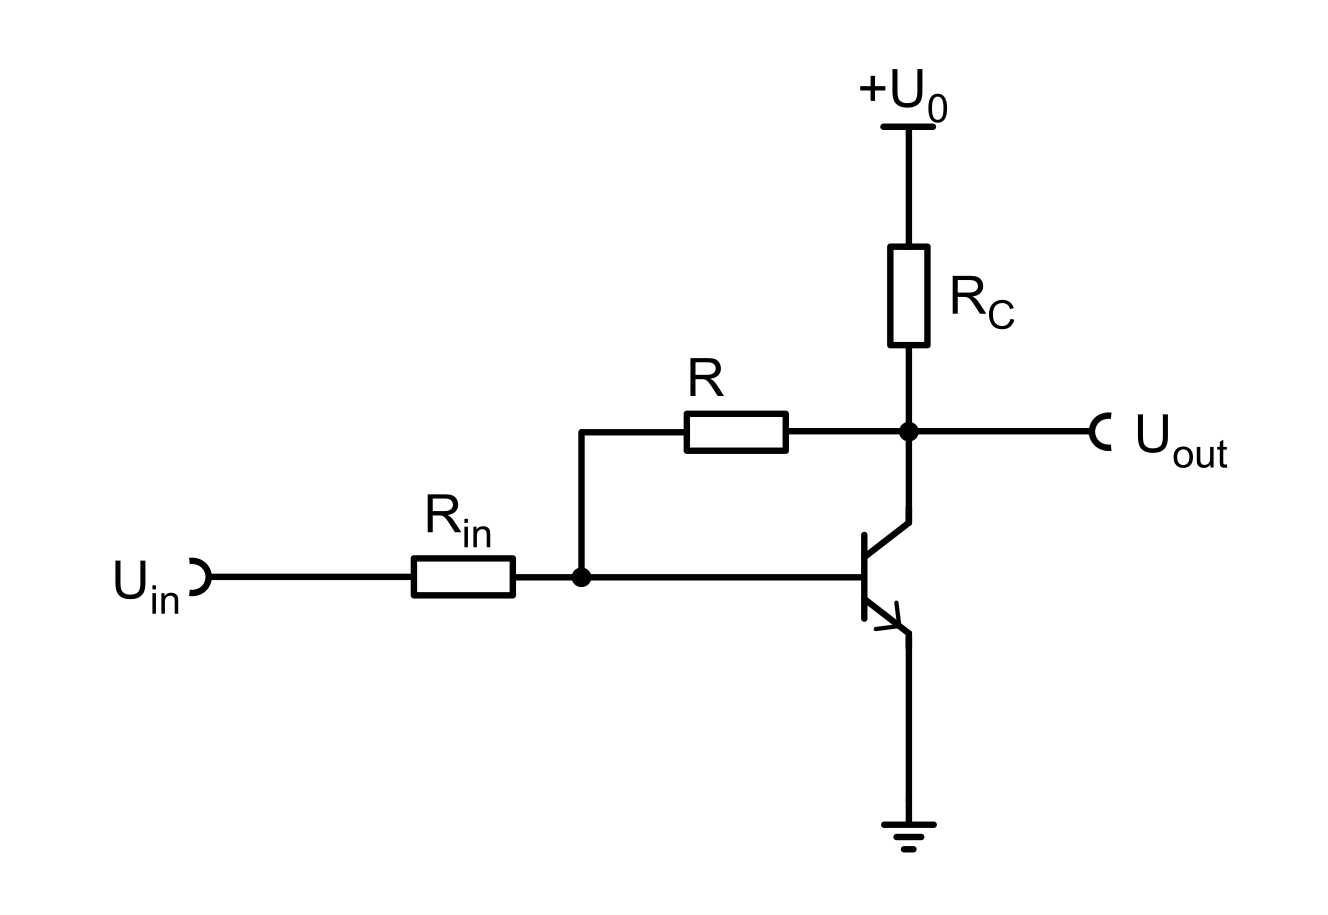
\includegraphics[width=0.6\textwidth]{spannungsgegenkopplung.png}
		\captionof{figure}{Transistor amplifier as common collector with negative feedback (voltage); figure 3/4.16 \cite{Praktikumsanleitung}}
	\end{Figure}
	In this figure the resistor $R$ sets the base potential as well as the operating point and couples the voltage from the collector back to the base.
	Due to this negative feedback the base current is reduced although the input current remains constant.

	\newpage
	\section{Preliminary Tasks}
	\subsection{G}
	$\zz\ \nu =\tfrac{\gamma R_E}{r_{BE}+\gamma R_E}$ with $\gamma =\diff[]{I_E}{I_B}$ and $r_{BE}=\diff[]{U_{BE}}{I_B}$.
	\begin{align}
		                &  & \nu & = \diff[]{U_E}{U_B}                                                    &  &           \\
		\Leftrightarrow &  &     & = \dfrac{\td I_ER_E}{\td U_{BE}+\td U_E}                               &  & \nonumber \\
		\Leftrightarrow &  &     & = \dfrac{\diff[]{I_ER_E}{I_B}}{\diff[]{U_{BE}}{I_B}+\diff[]{U_E}{I_B}} &  & \nonumber \\
		\Leftrightarrow &  &     & = \dfrac{\gamma R_E}{r_{BE}+\gamma R_E}.                               &  &
	\end{align}

	\subsection{H}
	The equation applies
	\begin{align}
		                &  & \dfrac{r_\text{out}}{r_\text{in}} & = \dfrac{\diff[]{U_E}{I_E}}{\diff[]{U_B}{I_B}} &  &           \\
		\Leftrightarrow &  &                                   & = \diff[]{U_E}{I_E}\diff[]{I_B}{U_B}           &  & \nonumber \\
		\Leftrightarrow &  &                                   & = \diff[]{U_E}{U_B}\diff[]{I_B}{I_E}           &  & \nonumber \\
		\Leftrightarrow &  &                                   & \approx 1\cdot \dfrac{1}{\gamma }.             &  &
	\end{align}

	\subsection{I}
	The equation applies
	\begin{align}
		                &  & \nu & = \diff[]{U_C}{U_B}                                                    &  &           \\
		\Leftrightarrow &  &     & = \dfrac{\td I_CR_C}{\td U_{BE}+\td U_E}                               &  & \nonumber \\
		\Leftrightarrow &  &     & = \dfrac{\diff[]{I_CR_C}{I_B}}{\diff[]{U_{BE}}{I_B}+\diff[]{U_E}{I_B}} &  & \nonumber \\
		\Leftrightarrow &  &     & = \dfrac{\beta R_C}{r_{BE}+\gamma R_E}.                                &  &
	\end{align}

	\subsection{J}
	The equation applies
	\begin{align}
		                &  & \dfrac{1}{\nu}       & = \tfrac{1+k\nu _0}{\nu _0}                   &  &           \\
		\Leftrightarrow &  & \nu                  & = \dfrac{\nu_0}{1+k\nu_0}                     &  & \nonumber \\
		\Leftrightarrow &  & \diff[]{\nu}{\nu_0}  & = \dfrac{1}{\left(1+k\nu_0\right)^2}          &  & \nonumber \\
		\Leftrightarrow &  &                      & = \dfrac{\nu}{\nu_0}\dfrac{1}{1+k\nu_0}       &  & \nonumber \\
		\Leftrightarrow &  & \dfrac{\td \nu}{\nu} & = \dfrac{\td \nu_0}{\nu_0}\dfrac{1}{1+k\nu_0} &  & \nonumber \\
		\Leftrightarrow &  &                      & = \dfrac{\td \nu_0}{\nu_0}\dfrac{\nu}{\nu_0}. &  &
	\end{align}

	\subsection{K}
	The parallel capacitor with capacitance $C_{CB}$ and transistor form a high--pass filter.
	This means that high frequency signals will run through the capacitor and not the transistor, resulting in them not being amplified.

	\subsection{L}
	There is no voltage change at point P, because the input signal to the transistor T2 is constant.
	The change in current $\td I_E\left(T_2\right)$ is in return also zero.

	\subsection{M}
	For any transit frequency the equation holds $f_\text{grenz gk}\nu\left(f=0\right)=f_\text{grenz}\nu_0$.
	Thus $f_\text{grenz gk}=f_\text{grenz}\tfrac{\nu_0}{\nu\left(f=0\right)}$.

	\subsection{N}
	For increasing base current $I_B$, the collector voltage $U_C$ and the voltage across the resistor $U_{R_C}$ also increases.
	Because $U_0$ should be constant, the voltage drops across the resistor $R$, which in turn stabilizes the operating point.

	\clearpage
	\section{Analysis}
	\subsection{Voltageamplifier of the common collector}
	On circut board I (Fig. \ref{fig:cb1}) we construct a common collector with d$U_B=\SI{2.1}{V_{PP}}$ and $U_B\approx \SI{2}{V}$. To test the voltage ampilification we chose a variety of diffrent resistor combinations. The messurements are displayed in Tab. \ref{tab:voltage_amplification}. We expect no change for diffrent $R_E$.
	\begin{Figure}
		\centering
		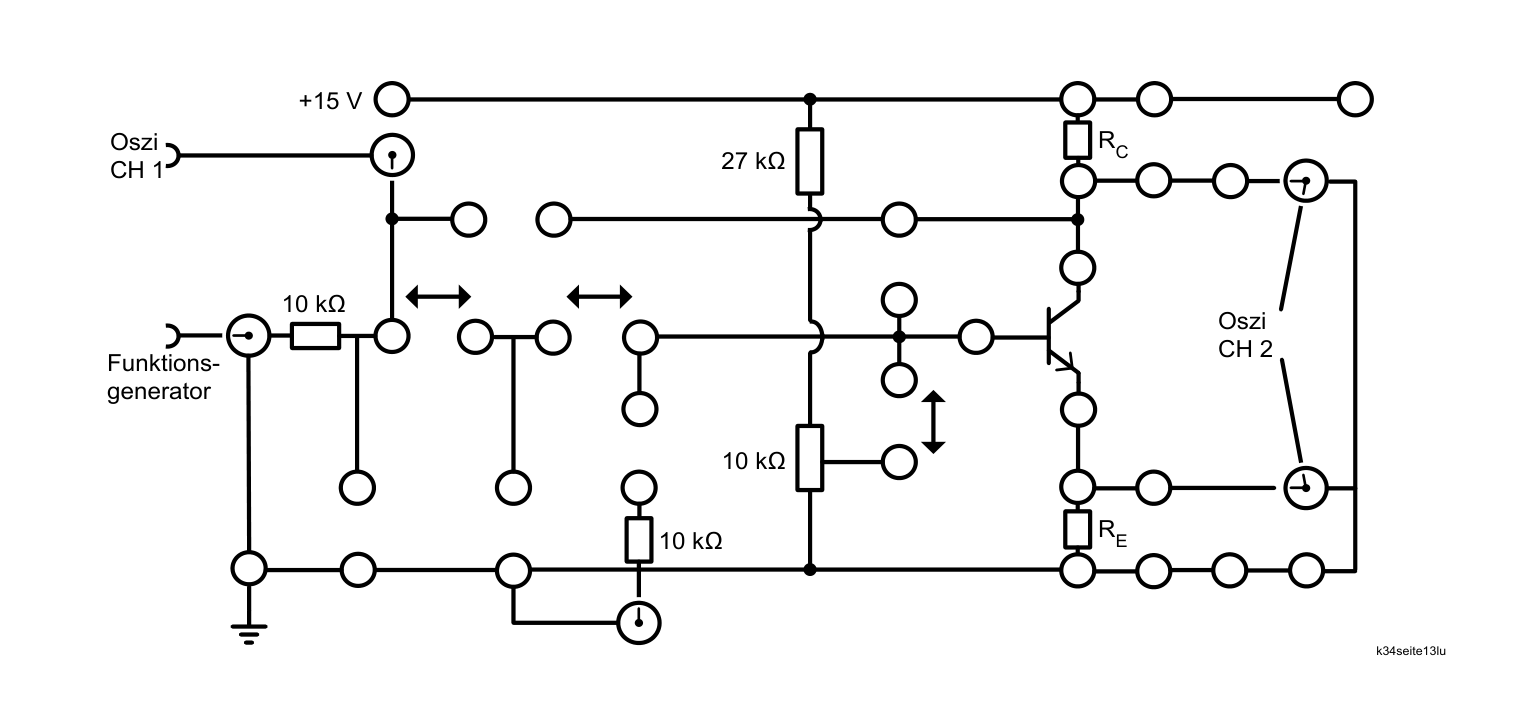
\includegraphics[width=1\textwidth]{circut_board_1.png}
		\captionof{figure}{Circut board 1\cite{Praktikumsanleitung}}
		\label{fig:cb1}
	\end{Figure}
	\begin{center}
		\begin{tabular}{|c|c|c|}
			\hline
			$R_C$            & $R_E$            & amplification $\nu$ \\
			\hline
			\SI{360}{\Omega} & \SI{1}{k\Omega}  & \SI{1+-0.025}{}     \\
			\SI{360}{\Omega} & \SI{22}{k\Omega} & \SI{1.025+-0.025}{} \\
			\SI{360}{\Omega} & \SI{47}{k\Omega} & \SI{1.015+-0.025}{} \\
			\hline
			\SI{1}{k\Omega}  & \SI{360}{\Omega} & \SI{0.945+-0.025}{} \\
			\SI{22}{k\Omega} & \SI{360}{\Omega} & \SI{0.114+-0.025}{} \\
			\SI{47}{k\Omega} & \SI{360}{\Omega} & \SI{0.12+-0.025}{}  \\
			\hline
		\end{tabular}
		\captionof{table}{Voltage amplification for diffrent resistor combinations}
		\label{tab:voltage_amplification}
	\end{center}
	As we see, there is no significant variation of the amplification for diffrent $R_E$. Though we can clearly see a lowering of the amplification for higher $R_C$, wich is plausible since we have less current that can be amplified.


	\subsection{Common collector as buffer amplifier}
	Here we are tasked to match the impedance of a speaker, so we are able to hear an output. For this we firstly construct an Inverted Amplifiert and test the speaker solely without a common collector. We observe, that the speaker does not produce any sound, because we havent matched the impedance. Now we add a common collecter as a buffer amplifier, wich in theroy should be able to match the impedance of the speaker. Unfortunatly we could not get the circut running and test the hypothisis.

	\subsection{Inverted amplifier}
	\subsubsection*{Phasere relationship between input and output}
	Now we build a common emitter on circut board I with $R_C=R_E=\SI{390}{\Omega}$, d$U_B=\SI{0.5}{V_{PP}}$, $U_B=\SI{1.5}{V}$ and we choose a capacity prior to the input signal of \SI{0.1}{\micro F}. As we can see in the xy (CH1, CH2) configuration in fig. \ref{fig:phasexy}, the phase is not linear, but eliptic. Thus we have not the same phase. We found out through experimenting, that the multiple elipsis come from noise. The phase relationship and especially the noise is also visible in fig. \ref{fig:phase}, as the lines are rather thicc. We can see that the phase diffrence is between $\frac{1}{2}\pi$ and $1\pi$, because we now have coupled the capacitor.
	\begin{Figure}
		\centering
		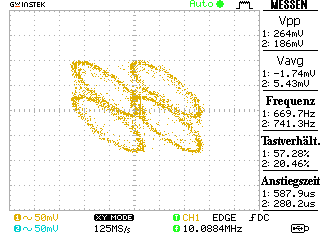
\includegraphics[width=1\textwidth]{../data/DS0020.png}
		\captionof{figure}{Phase relationship in phase space}
		\label{fig:phasexy}
	\end{Figure}
	\begin{Figure}
		\centering
		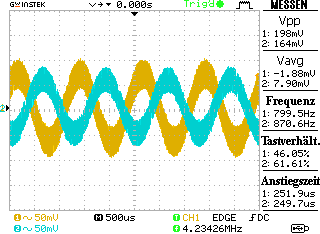
\includegraphics[width=1\textwidth]{../data/DS0021.png}
		\captionof{figure}{Phase relationship in voltage/time space}
		\label{fig:phase}
	\end{Figure}
	\subsubsection*{Voltage amplification of the inverted amplifier}
	We measure the voltage amplification with diffrent values for the resistors $R_E$ and $R_C$. The results are display in tab. \ref{tab:voltage_amplification2}.
	\begin{center}
		\begin{tabular}{|c|c|c|c|}
			\hline
			$R_C$             & $R_E$             & amplification $\nu$  & $\nu = -\frac{R_C}{R_E}$ \\
			\hline
			\SI{360}{\Omega}  & \SI{470}{\Omega}  & \SI{-0.686+-0.024}{} & -0.830                   \\
			\SI{360}{\Omega}  & \SI{1}{k\Omega}   & \SI{-0.437+-0.024}{} & -0.390                   \\
			\SI{360}{\Omega}  & \SI{4.7}{k\Omega} & \SI{-0.25+-0.025}{}  & -0.083                   \\
			\SI{360}{\Omega}  & \SI{33}{k\Omega}  & \SI{-0.196+-0.025}{} & -0.012                   \\
			\SI{360}{\Omega}  & \SI{47}{k\Omega}  & \SI{-0.18+-0.025}{}  & -0.008                   \\
			\hline
			\SI{470}{\Omega}  & \SI{360}{\Omega}  & \SI{-0.857+-0.024}{} & -1.205                   \\
			\SI{1}{k\Omega}   & \SI{360}{\Omega}  & \SI{-1.491+-0.025}{} & -2.564                   \\
			\SI{4.7}{k\Omega} & \SI{360}{\Omega}  & \SI{-2.284+-0.022}{} & -12.05                   \\
			\SI{33}{k\Omega}  & \SI{360}{\Omega}  & \SI{-0.234+-0.027}{} & -84.62                   \\
			\SI{47}{k\Omega}  & \SI{360}{\Omega}  & \SI{-0.234+-0.027}{} & -120.5                   \\
			\hline
		\end{tabular}
		\captionof{table}{Voltage amplification for diffrent resistor combinations}
		\label{tab:voltage_amplification2}
	\end{center}
	We notice, where $R_C$ stays constant, the experimental values for the amplification follow the theoretical ones in thier generall trend, but are not exactly the same. Where $R_E$ stays constant we observe that first the data follows the calculations, but to the end, with the highest restance, they just drop. It seems that there is a sweetspot for an optimal amplification. Then it should have to do something with resonace, so the amplification is frequency dependent. But since we expect that the formular for the theoreticle values is correct, we assume we have made some mistake for the last two experimental values.

	\subsubsection*{Resistance of a Transistor}
	Now with the special case, that $R_E=\SI{0}{\Omega}$ and $E_C=\SI{390}{\Omega}$, we can read the peak-to-peak voltage from oscillogramm in fig. \ref{fig:rn} and calculate the amplification. We calculate the amplification to be $\nu_0=\SI{-26.8+-1.0}{}$. $\beta=\SI{547+-27}{}$ has allready been determent in the last lab course. Now we can calculate the differential resistance of the Emitter-Base-Diod $r_{BE}$:
	\begin{align*}
		\nu_0                  & =-\beta\frac{R_C}{r_{BE}}     \\
		\Leftrightarrow r_{BE} & =-\beta\frac{R_C}{\nu_0}      \\
		                       & =\SI{7.96+-0.49}{\kilo\Omega}
	\end{align*}
	.
	\begin{Figure}
		\centering
		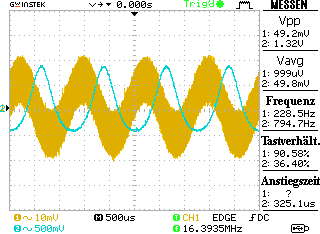
\includegraphics[width=1\textwidth]{../data/DS0022.png}
		\captionof{figure}{Voltage amplification}
		\label{fig:rn}
	\end{Figure}
	We now plot the data from tab. \ref{tab:voltage_amplification2} in fig. \ref{fig:rcconst} and \ref{fig:reconst}. At this point we are tasked to display the theoretical line in the figures, however they diverge to the extend, that one of them would not be readable anymore. So we choose not to display the theoretical line, but rather the fit we have done to our data. As mentioned previously, the two last data points are probably not representative in any way, so they will be left out.
	\begin{Figure}
		\centering\resizebox{\textwidth}{!}{% GNUPLOT: LaTeX picture with Postscript
\begingroup
  \makeatletter
  \providecommand\color[2][]{%
    \GenericError{(gnuplot) \space\space\space\@spaces}{%
      Package color not loaded in conjunction with
      terminal option `colourtext'%
    }{See the gnuplot documentation for explanation.%
    }{Either use 'blacktext' in gnuplot or load the package
      color.sty in LaTeX.}%
    \renewcommand\color[2][]{}%
  }%
  \providecommand\includegraphics[2][]{%
    \GenericError{(gnuplot) \space\space\space\@spaces}{%
      Package graphicx or graphics not loaded%
    }{See the gnuplot documentation for explanation.%
    }{The gnuplot epslatex terminal needs graphicx.sty or graphics.sty.}%
    \renewcommand\includegraphics[2][]{}%
  }%
  \providecommand\rotatebox[2]{#2}%
  \@ifundefined{ifGPcolor}{%
    \newif\ifGPcolor
    \GPcolortrue
  }{}%
  \@ifundefined{ifGPblacktext}{%
    \newif\ifGPblacktext
    \GPblacktexttrue
  }{}%
  % define a \g@addto@macro without @ in the name:
  \let\gplgaddtomacro\g@addto@macro
  % define empty templates for all commands taking text:
  \gdef\gplbacktext{}%
  \gdef\gplfronttext{}%
  \makeatother
  \ifGPblacktext
    % no textcolor at all
    \def\colorrgb#1{}%
    \def\colorgray#1{}%
  \else
    % gray or color?
    \ifGPcolor
      \def\colorrgb#1{\color[rgb]{#1}}%
      \def\colorgray#1{\color[gray]{#1}}%
      \expandafter\def\csname LTw\endcsname{\color{white}}%
      \expandafter\def\csname LTb\endcsname{\color{black}}%
      \expandafter\def\csname LTa\endcsname{\color{black}}%
      \expandafter\def\csname LT0\endcsname{\color[rgb]{1,0,0}}%
      \expandafter\def\csname LT1\endcsname{\color[rgb]{0,1,0}}%
      \expandafter\def\csname LT2\endcsname{\color[rgb]{0,0,1}}%
      \expandafter\def\csname LT3\endcsname{\color[rgb]{1,0,1}}%
      \expandafter\def\csname LT4\endcsname{\color[rgb]{0,1,1}}%
      \expandafter\def\csname LT5\endcsname{\color[rgb]{1,1,0}}%
      \expandafter\def\csname LT6\endcsname{\color[rgb]{0,0,0}}%
      \expandafter\def\csname LT7\endcsname{\color[rgb]{1,0.3,0}}%
      \expandafter\def\csname LT8\endcsname{\color[rgb]{0.5,0.5,0.5}}%
    \else
      % gray
      \def\colorrgb#1{\color{black}}%
      \def\colorgray#1{\color[gray]{#1}}%
      \expandafter\def\csname LTw\endcsname{\color{white}}%
      \expandafter\def\csname LTb\endcsname{\color{black}}%
      \expandafter\def\csname LTa\endcsname{\color{black}}%
      \expandafter\def\csname LT0\endcsname{\color{black}}%
      \expandafter\def\csname LT1\endcsname{\color{black}}%
      \expandafter\def\csname LT2\endcsname{\color{black}}%
      \expandafter\def\csname LT3\endcsname{\color{black}}%
      \expandafter\def\csname LT4\endcsname{\color{black}}%
      \expandafter\def\csname LT5\endcsname{\color{black}}%
      \expandafter\def\csname LT6\endcsname{\color{black}}%
      \expandafter\def\csname LT7\endcsname{\color{black}}%
      \expandafter\def\csname LT8\endcsname{\color{black}}%
    \fi
  \fi
    \setlength{\unitlength}{0.0500bp}%
    \ifx\gptboxheight\undefined%
      \newlength{\gptboxheight}%
      \newlength{\gptboxwidth}%
      \newsavebox{\gptboxtext}%
    \fi%
    \setlength{\fboxrule}{0.5pt}%
    \setlength{\fboxsep}{1pt}%
    \definecolor{tbcol}{rgb}{1,1,1}%
\begin{picture}(7200.00,4320.00)%
    \gplgaddtomacro\gplbacktext{%
      \csname LTb\endcsname%%
      \put(536,619){\makebox(0,0)[r]{\strut{}$-7$}}%
      \csname LTb\endcsname%%
      \put(536,1135){\makebox(0,0)[r]{\strut{}$-6$}}%
      \csname LTb\endcsname%%
      \put(536,1652){\makebox(0,0)[r]{\strut{}$-5$}}%
      \csname LTb\endcsname%%
      \put(536,2169){\makebox(0,0)[r]{\strut{}$-4$}}%
      \csname LTb\endcsname%%
      \put(536,2686){\makebox(0,0)[r]{\strut{}$-3$}}%
      \csname LTb\endcsname%%
      \put(536,3202){\makebox(0,0)[r]{\strut{}$-2$}}%
      \csname LTb\endcsname%%
      \put(536,3719){\makebox(0,0)[r]{\strut{}$-1$}}%
      \csname LTb\endcsname%%
      \put(634,425){\makebox(0,0){\strut{}$0$}}%
      \csname LTb\endcsname%%
      \put(1259,425){\makebox(0,0){\strut{}$5000$}}%
      \csname LTb\endcsname%%
      \put(1884,425){\makebox(0,0){\strut{}$10000$}}%
      \csname LTb\endcsname%%
      \put(2509,425){\makebox(0,0){\strut{}$15000$}}%
      \csname LTb\endcsname%%
      \put(3134,425){\makebox(0,0){\strut{}$20000$}}%
      \csname LTb\endcsname%%
      \put(3760,425){\makebox(0,0){\strut{}$25000$}}%
      \csname LTb\endcsname%%
      \put(4385,425){\makebox(0,0){\strut{}$30000$}}%
      \csname LTb\endcsname%%
      \put(5010,425){\makebox(0,0){\strut{}$35000$}}%
      \csname LTb\endcsname%%
      \put(5635,425){\makebox(0,0){\strut{}$40000$}}%
      \csname LTb\endcsname%%
      \put(6261,425){\makebox(0,0){\strut{}$45000$}}%
      \csname LTb\endcsname%%
      \put(6886,425){\makebox(0,0){\strut{}$50000$}}%
    }%
    \gplgaddtomacro\gplfronttext{%
      \csname LTb\endcsname%%
      \put(6123,3545){\makebox(0,0)[r]{\strut{}data}}%
      \csname LTb\endcsname%%
      \put(6123,3351){\makebox(0,0)[r]{\strut{}$\frac{1}{v(R_E)}_{fit} = \frac{1}{v_0} - \frac{1}{R_C} \cdot R_E$}}%
      \csname LTb\endcsname%%
      \put(170,2169){\rotatebox{-270.00}{\makebox(0,0){\strut{}$\frac{1}{\nu}$}}}%
      \csname LTb\endcsname%%
      \put(3760,135){\makebox(0,0){\strut{}$R_E$ [$\Omega$]}}%
      \csname LTb\endcsname%%
      \put(3760,4009){\makebox(0,0){\strut{}Amplification resistance relation with constant R_C}}%
    }%
    \gplbacktext
    \put(0,0){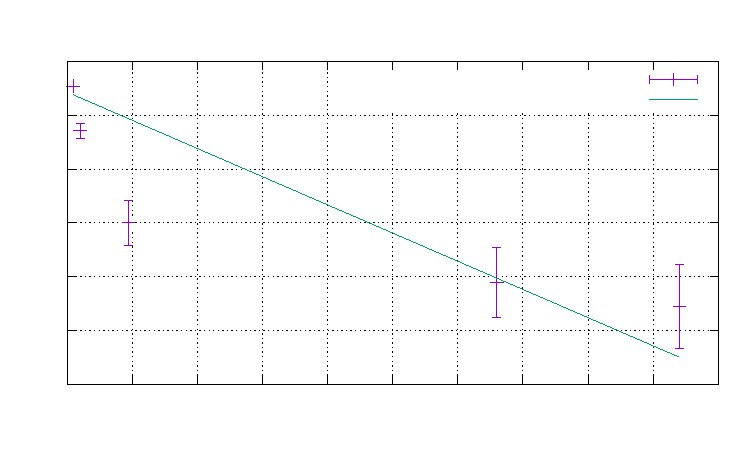
\includegraphics[width={360.00bp},height={216.00bp}]{amp_res_relation}}%
    \gplfronttext
  \end{picture}%
\endgroup
}
		\captionof{figure}{Amplification-Resistance-Relation for constant $R_C$}
		\label{fig:rcconst}
	\end{Figure}
	\begin{Figure}
		\centering\resizebox{\textwidth}{!}{% GNUPLOT: LaTeX picture with Postscript
\begingroup
  \makeatletter
  \providecommand\color[2][]{%
    \GenericError{(gnuplot) \space\space\space\@spaces}{%
      Package color not loaded in conjunction with
      terminal option `colourtext'%
    }{See the gnuplot documentation for explanation.%
    }{Either use 'blacktext' in gnuplot or load the package
      color.sty in LaTeX.}%
    \renewcommand\color[2][]{}%
  }%
  \providecommand\includegraphics[2][]{%
    \GenericError{(gnuplot) \space\space\space\@spaces}{%
      Package graphicx or graphics not loaded%
    }{See the gnuplot documentation for explanation.%
    }{The gnuplot epslatex terminal needs graphicx.sty or graphics.sty.}%
    \renewcommand\includegraphics[2][]{}%
  }%
  \providecommand\rotatebox[2]{#2}%
  \@ifundefined{ifGPcolor}{%
    \newif\ifGPcolor
    \GPcolortrue
  }{}%
  \@ifundefined{ifGPblacktext}{%
    \newif\ifGPblacktext
    \GPblacktexttrue
  }{}%
  % define a \g@addto@macro without @ in the name:
  \let\gplgaddtomacro\g@addto@macro
  % define empty templates for all commands taking text:
  \gdef\gplbacktext{}%
  \gdef\gplfronttext{}%
  \makeatother
  \ifGPblacktext
    % no textcolor at all
    \def\colorrgb#1{}%
    \def\colorgray#1{}%
  \else
    % gray or color?
    \ifGPcolor
      \def\colorrgb#1{\color[rgb]{#1}}%
      \def\colorgray#1{\color[gray]{#1}}%
      \expandafter\def\csname LTw\endcsname{\color{white}}%
      \expandafter\def\csname LTb\endcsname{\color{black}}%
      \expandafter\def\csname LTa\endcsname{\color{black}}%
      \expandafter\def\csname LT0\endcsname{\color[rgb]{1,0,0}}%
      \expandafter\def\csname LT1\endcsname{\color[rgb]{0,1,0}}%
      \expandafter\def\csname LT2\endcsname{\color[rgb]{0,0,1}}%
      \expandafter\def\csname LT3\endcsname{\color[rgb]{1,0,1}}%
      \expandafter\def\csname LT4\endcsname{\color[rgb]{0,1,1}}%
      \expandafter\def\csname LT5\endcsname{\color[rgb]{1,1,0}}%
      \expandafter\def\csname LT6\endcsname{\color[rgb]{0,0,0}}%
      \expandafter\def\csname LT7\endcsname{\color[rgb]{1,0.3,0}}%
      \expandafter\def\csname LT8\endcsname{\color[rgb]{0.5,0.5,0.5}}%
    \else
      % gray
      \def\colorrgb#1{\color{black}}%
      \def\colorgray#1{\color[gray]{#1}}%
      \expandafter\def\csname LTw\endcsname{\color{white}}%
      \expandafter\def\csname LTb\endcsname{\color{black}}%
      \expandafter\def\csname LTa\endcsname{\color{black}}%
      \expandafter\def\csname LT0\endcsname{\color{black}}%
      \expandafter\def\csname LT1\endcsname{\color{black}}%
      \expandafter\def\csname LT2\endcsname{\color{black}}%
      \expandafter\def\csname LT3\endcsname{\color{black}}%
      \expandafter\def\csname LT4\endcsname{\color{black}}%
      \expandafter\def\csname LT5\endcsname{\color{black}}%
      \expandafter\def\csname LT6\endcsname{\color{black}}%
      \expandafter\def\csname LT7\endcsname{\color{black}}%
      \expandafter\def\csname LT8\endcsname{\color{black}}%
    \fi
  \fi
    \setlength{\unitlength}{0.0500bp}%
    \ifx\gptboxheight\undefined%
      \newlength{\gptboxheight}%
      \newlength{\gptboxwidth}%
      \newsavebox{\gptboxtext}%
    \fi%
    \setlength{\fboxrule}{0.5pt}%
    \setlength{\fboxsep}{1pt}%
    \definecolor{tbcol}{rgb}{1,1,1}%
\begin{picture}(7200.00,4320.00)%
    \gplgaddtomacro\gplbacktext{%
      \csname LTb\endcsname%%
      \put(731,619){\makebox(0,0)[r]{\strut{}$-2.5$}}%
      \csname LTb\endcsname%%
      \put(731,1239){\makebox(0,0)[r]{\strut{}$-2$}}%
      \csname LTb\endcsname%%
      \put(731,1859){\makebox(0,0)[r]{\strut{}$-1.5$}}%
      \csname LTb\endcsname%%
      \put(731,2479){\makebox(0,0)[r]{\strut{}$-1$}}%
      \csname LTb\endcsname%%
      \put(731,3099){\makebox(0,0)[r]{\strut{}$-0.5$}}%
      \csname LTb\endcsname%%
      \put(731,3719){\makebox(0,0)[r]{\strut{}$0$}}%
      \csname LTb\endcsname%%
      \put(829,425){\makebox(0,0){\strut{}$0$}}%
      \csname LTb\endcsname%%
      \put(1435,425){\makebox(0,0){\strut{}$500$}}%
      \csname LTb\endcsname%%
      \put(2041,425){\makebox(0,0){\strut{}$1000$}}%
      \csname LTb\endcsname%%
      \put(2646,425){\makebox(0,0){\strut{}$1500$}}%
      \csname LTb\endcsname%%
      \put(3252,425){\makebox(0,0){\strut{}$2000$}}%
      \csname LTb\endcsname%%
      \put(3858,425){\makebox(0,0){\strut{}$2500$}}%
      \csname LTb\endcsname%%
      \put(4463,425){\makebox(0,0){\strut{}$3000$}}%
      \csname LTb\endcsname%%
      \put(5069,425){\makebox(0,0){\strut{}$3500$}}%
      \csname LTb\endcsname%%
      \put(5674,425){\makebox(0,0){\strut{}$4000$}}%
      \csname LTb\endcsname%%
      \put(6280,425){\makebox(0,0){\strut{}$4500$}}%
      \csname LTb\endcsname%%
      \put(6886,425){\makebox(0,0){\strut{}$5000$}}%
    }%
    \gplgaddtomacro\gplfronttext{%
      \csname LTb\endcsname%%
      \put(6123,3545){\makebox(0,0)[r]{\strut{}data}}%
      \csname LTb\endcsname%%
      \put(6123,3351){\makebox(0,0)[r]{\strut{}$v_{fit}(R_C) = - k \cdot R_C$ with $k=\frac{\beta}{r_{BE} + \gamma R_E}$}}%
      \csname LTb\endcsname%%
      \put(170,2169){\rotatebox{-270.00}{\makebox(0,0){\strut{}$\nu$}}}%
      \csname LTb\endcsname%%
      \put(3858,135){\makebox(0,0){\strut{}$R_C$ [$\Omega$]}}%
      \csname LTb\endcsname%%
      \put(3858,4009){\makebox(0,0){\strut{}Amplification resistance relation wiht constant R_E}}%
    }%
    \gplbacktext
    \put(0,0){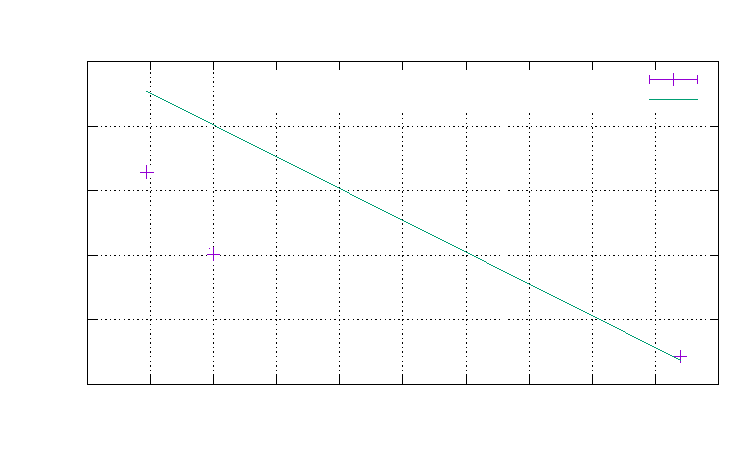
\includegraphics[width={360.00bp},height={216.00bp}]{amp_res_relation2}}%
    \gplfronttext
  \end{picture}%
\endgroup
}
		\captionof{figure}{Amplification-Resistance-Relation for constant $R_E$}
		\label{fig:reconst}
	\end{Figure}
	\begin{center}
		\begin{tabular}{|c|c|}
			\hline
			Paramter & Value                      \\
			\hline
			$\nu_0$  & \SI{-0.639+-0.095}{}       \\
			$R_C$    & \SI{9.5+-4.7}{\kilo\Omega} \\
			\hline
		\end{tabular}
		\captionof{table}{Fit-Paramter und Werte}
		\label{tab:1.1}
	\end{center}
	\begin{center}
		\begin{tabular}{|c|c|}
			\hline
			Paramter & Value                                \\
			\hline
			k        & \SI{492+-58}{\micro\frac{1}{\Omega}} \\
			\hline
		\end{tabular}
		\captionof{table}{Fit-Paramter und Werte}
		\label{tab:1.2}
	\end{center}
	We have got the values for the parameters presented in tab. \ref{tab:1.1} and \ref{tab:1.2}. Here we use
	\begin{align*}
		\frac{1}{v}(R_E) & = \frac{1}{v_0} - \frac{1}{R_C} \cdot R_E \text{ and}    \\
		v(R_C)           & = - k \cdot R_C                                          \\
		                 & \text{with }k=\frac{\beta}{r_{BE} + \gamma R_E} \text{.}
	\end{align*}
	When comparing $\nu_0$, $R_C$ and $k$ to the previous calculated/set values, it is obvius that no fittet values are anywhere near the expected range or order. This is probably a consequence of bad execution of the experiment. Now, without the constructed circut, it is not easy to tell afterwards where exact our mistake took place. We noticed a lot of noice thoughout the whole lab course, that sometimes could be fixed, or at least fixed to an extend, by moving our connections or holding them in spesific but seemingly random places. So another source of error could have been the equipment, though we think with the right execution we would have gotten significant better results.

	\subsection{Alternating current cancellation of negative feedback}
	In this task, the noise visible on the oszillograph is reduced by increasing the voltage of the input signal.
	\\\\Changing $R_E$ to be zero, the amplification $|\nu |$ is maximised.
	The range in which the transistor has enough voltage to output a sinusoidal signal, meaning the signal lies within the dynamic range, is between $R_P  \in  \left[\SI{1.359}{k\ohm},\SI{3.161}{k\ohm}\right]$.
	$R_P$ is the potentiometer changing the offset voltage.
	For $R_E=\SI{390}{\ohm}$ (which is $|\nu |=1$), the potentiometer has a range of $R_P  \in  \left[\SI{1.178}{k\ohm},\SI{10}{k\ohm}=\text{max}\left(R_P\right)\right]$.
	\\\\Now a capacitor with capacitance $C=\SI{0.1}{\micro F}$ is connected in parallel with $R_E$.
	The previous amplification of around $10$ is achieved for a signal with frequency $\SI{44}{kHz}$.
	This makes sense, because the capacitor in parallel acts as a low pass, letting frequencies below $\SI{44}{kHz}$ pass through it, such that no amplification of 10 is achieved.
	The resistance above $\SI{44}{kHz}$ is high enough so that the signal passes through the transistor and gets amplified.

	\subsection{Frequency response of a cascode circuit}
	A \hyperref[fig:transistorverstärker]{transistor amplifier circuit} is constructed on \hyperref[fig:schaltbrett_2]{circuit board 2}.
	Output 2 is used here.
	\begin{Figure}
		\centering
		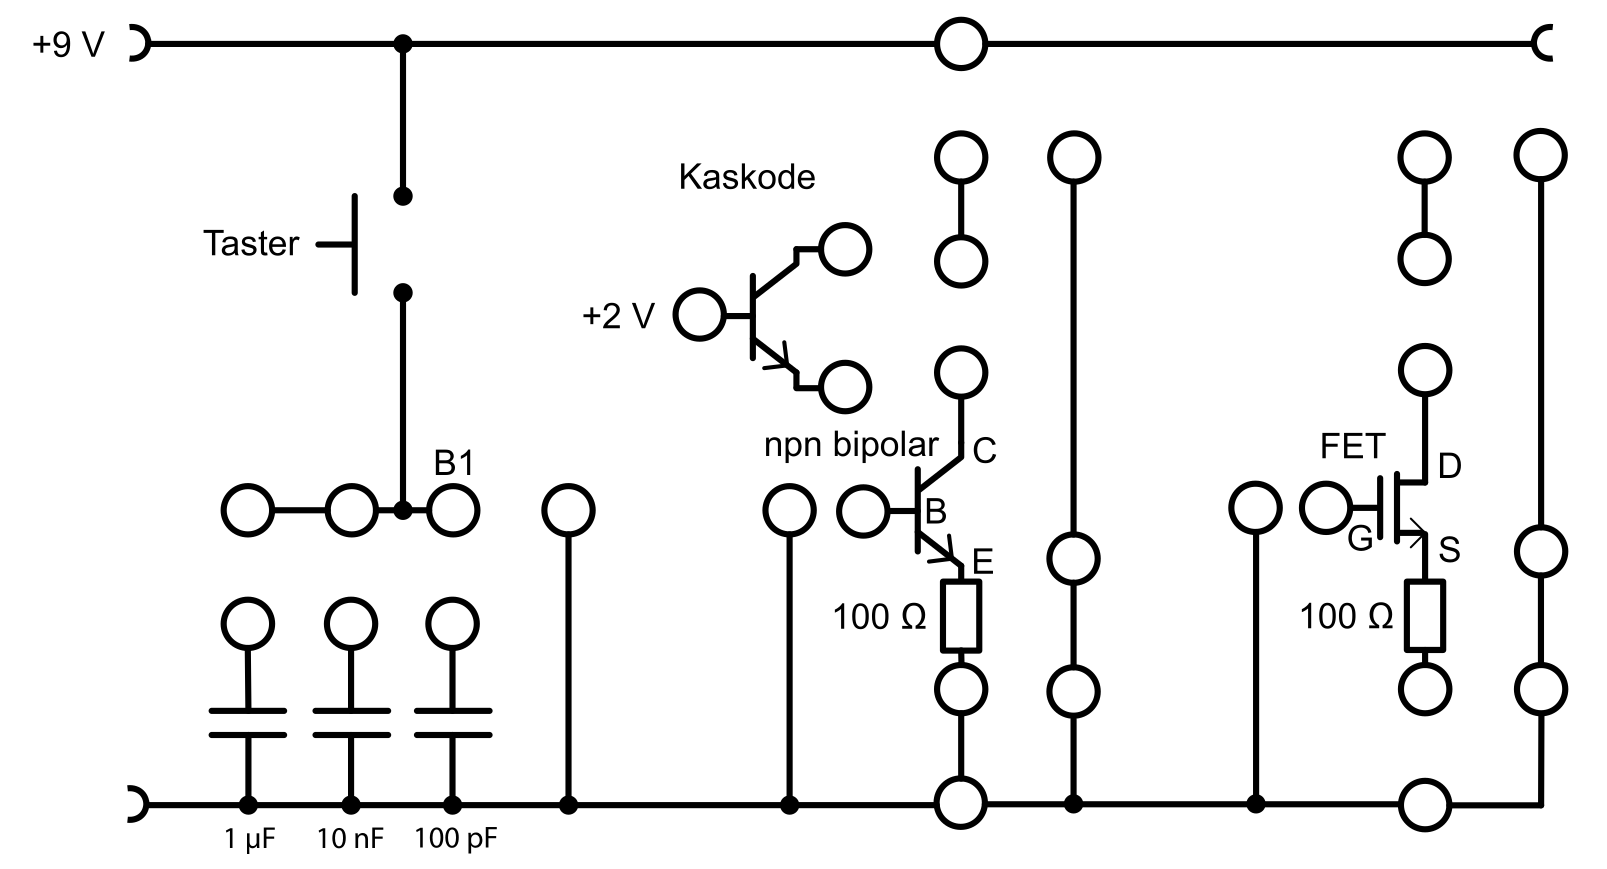
\includegraphics[width=0.6\textwidth]{schaltbrett_2.png}
		\captionof{figure}{Circuit board 2; Abb. 3.5\cite{Praktikumsanleitung}} \label{fig:schaltbrett_2}
	\end{Figure}
	\begin{Figure}
		\centering
		\includegraphics[width=0.6\textwidth]{transistorverstärker.png}
		\captionof{figure}{Transistor amplifier circuit using output 2; Abb. 3/4.15\cite{Praktikumsanleitung}} \label{fig:transistorverstärker}
	\end{Figure}
	To achieve an amplification of 10, the emitter and collector resistors are chosen to be $R_E=\SI{100}{\ohm}$ and $R_C=\SI{1}{k\ohm}=10\cdot R_E$.
	The input signal is a sinusoidal wave of $\SI{100}{Hz}$ with $U_{PP}=\SI{200}{mV}$.
	The DC--offset is set via a voltage divider.
	\begin{Figure}
		\centering
		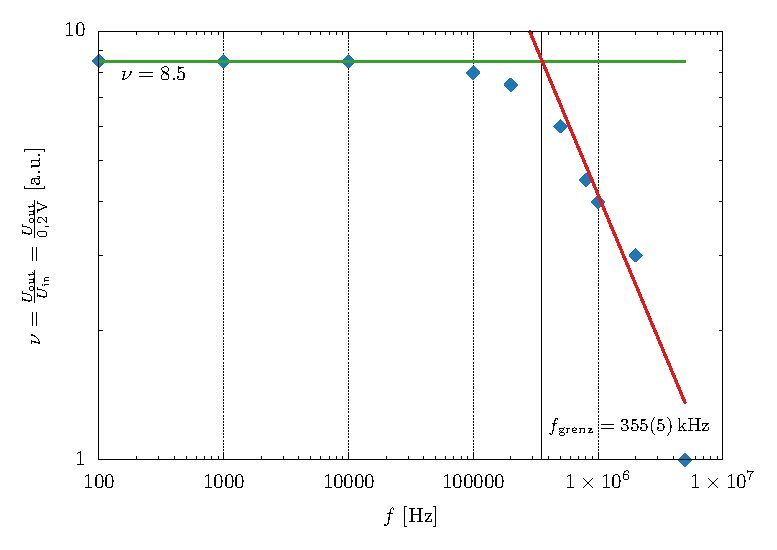
\includegraphics[width=\textwidth]{../plot/ex4_crop.pdf}
		\captionof{figure}{Bode--plot of a transistor amplifier circuit} \label{plot:bode}
	\end{Figure}
	\begin{center}
		\begin{tabular}{|c|c|c|}
			\hline
			frequency [Hz] & voltage [V] & $\nu$ [a.u.] \\
			\hline
			100            & 1.7         & 8.5          \\
			1000           & 1.7         & 8.5          \\
			10000          & 1.7         & 8.5          \\
			100000         & 1.6         & 8.0          \\
			200000         & 1.5         & 7.5          \\
			500000         & 1.2         & 6.0          \\
			800000         & 0.9         & 4.5          \\
			1000000        & 0.8         & 4.0          \\
			2000000        & 0.6         & 3.0          \\
			5000000        & 0.2         & 1.0          \\
			\hline
		\end{tabular}
		\captionof{table}{Values to \ref{plot:bode}}
	\end{center}
	The fit curve is given by $f\left(x\right)=x^m\cdot b$, with $m=\SI{-0.695813+-0.2463}{Hz^{-1}}$ and $b=\SI{62123.8+-2.149e+05}{}$.
	As expected, the amplification stays the same until the cutoff frequency $f_\text{grenz}=\SI{355+-5}{kHz}$ is reached.
	After that, the amplification decreases exponentially.
	At an amplification of $\nu =1$ the input voltage of $\SI{200}{mV}$ is reached.
	The transit frequency is calculated via
	\begin{align}
		f_T=f_\text{grenz}\nu _0=\SI{355+-5}{kHz}\cdot 8.5=\SI{3017.5+-42.5}{kHz}
		.\end{align}
	To calculate the bandwidth one can solve for $x$ in
	\begin{align}
		1=x^{m}\cdot b\quad \Leftrightarrow \quad x=B=\SI{7.73+-0.61}{MHz}
		.\end{align}
	Due to lack of time, it was not possible to construct the cacode circuit and measure the amplification--frequency relation again.
	Though it was expected to see a decline in amplification for an increase in bandwidth.
	The transit frequency would have still been the same.

	\subsection{Amplifier with negative feedback}
	Due to time contrains it was not possible to complete the final task.
	\begin{Figure}
		\centering
		\includegraphics[width=\textwidth]{verstärker_mit_spannungsgegenkopplung}
		\captionof{figure}{Amplifier with negative feedback; Abb. 4.1\cite{Praktikumsanleitung}}
	\end{Figure}
	With $R=\SI{100}{\kilo\ohm}$ as well as $R=\SI{33}{k\ohm}$ the voltage amplification $\diff[]{U_\text{out}}{U_\text{in}}$ should have been measured for an input frequency of $f=\SI{1}{kHz}$.
	\\\indent Because $R_\text{in}$ reduces the amplification, measurements have to be taken after $R_\text{in}$ as well.
	One would expect an increase in amplification because no voltage can drop across $R_\text{in}$.

	\section{Conclusion}
  In this lab course we have further explored the common collector as voltage amplifier. Furthermore we build a common collector as buffer amplifier with the example of a speaker. This was, due to some complications, sadly not possible to constuct, but the theory was still understood. After the common collector, we build a common emitter, wich acted as inverter amplifier. The inversion was nicely observed with Lissajous Figures. Aftwerards we treid to measure the amplification, wich was not quite possible. We took measuremnts but in the analysis it was quite quikly clear, that the results were not following the theory. But the measurements were still good enough to extract e.g. $\nu_0$ and directly see the discrepancy ($\nu_0=\SI{-26.8+-1.0}{}$ in comparison to the \SI{-0.639+-0.095}{} through the fitting). Also one could demonstrate the effect of an high--pass used in an amplifier, by connecting a capacitor in parallel and comparing the frequencies at which a similar amplification is achieved.
	\\\indent The cutoff frequency of an amplifier circuit is demonstrated in a bode--plot (\ref{plot:bode}).
	It can be seen that the amplification stays constant and suddenly falls at the cutoff frequency of $f_\text{grenz}=\SI{355+-5}{kHz}$.
	One can now calculate the transit frequency to be $f_T=\SI{3017.5+-42.5}{kHz}$ and the bandwidth $B=\SI{7.73+-0.61}{MHz}$.
	\\\indent Due to lack of time the comparison with a cascode circuit as well as the last task couldn't be completed.
	The expected results have been discussed nevertheless.

\end{multicols}

\clearpage
\listoffigures
\listoftables
\bibliographystyle{plain}
\bibliography{refs}

%}}}

\end{document}
